%!TEX root = ../../Principal/TFG.tex
\chapter{Anexo I: Calidad de las clasificaciones obtenidas en identificaci�n}
\label{appe:A}
\pagestyle{fancy}
\thispagestyle{empty}
%
\graphicspath{{../ApendiceA/Imagenes/}}
\DeclareGraphicsExtensions{.pdf,.png,.jpg}

% Empieza a escribir aqu�
\section{Base de datos 1}

\begin{table}[h]{
	\centering
	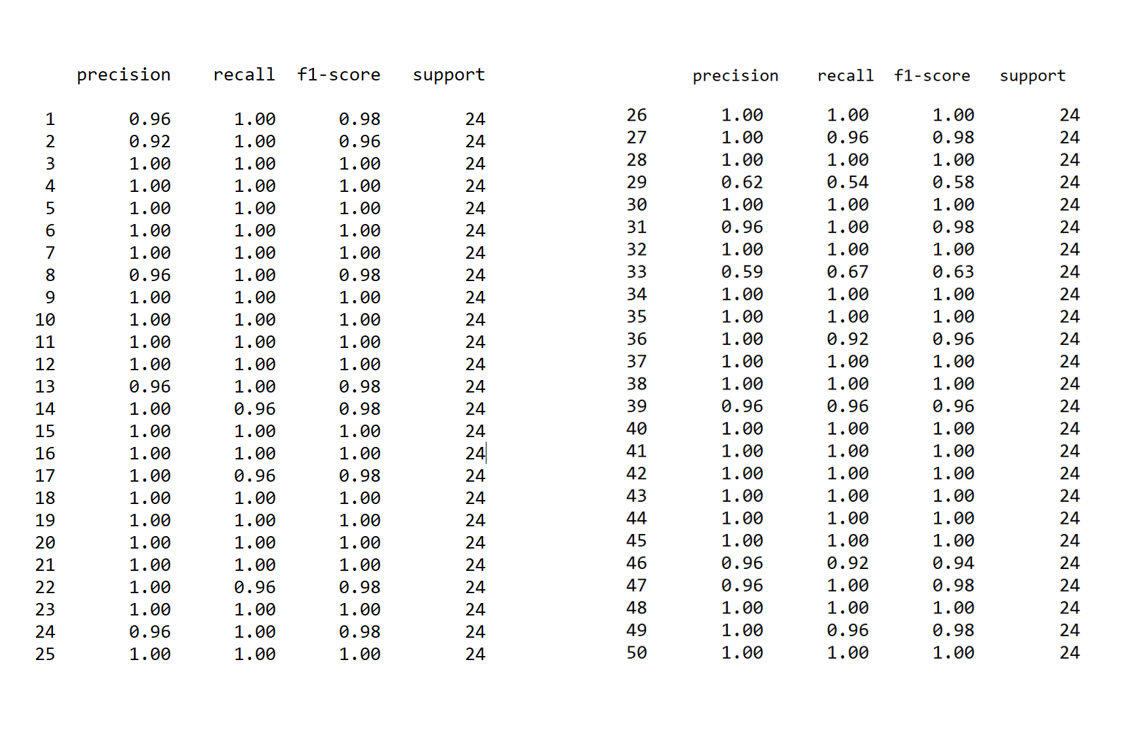
\includegraphics[width=1.1\textwidth]{/clasif1_}}
\caption{Calidad de las clasificaciones obtenidas para cada usuario de la primera base de datos.}
\label{clasif1}
\end{table}
\newpage

\section{Base de datos 2}


\begin{table}[h]{
		\centering
		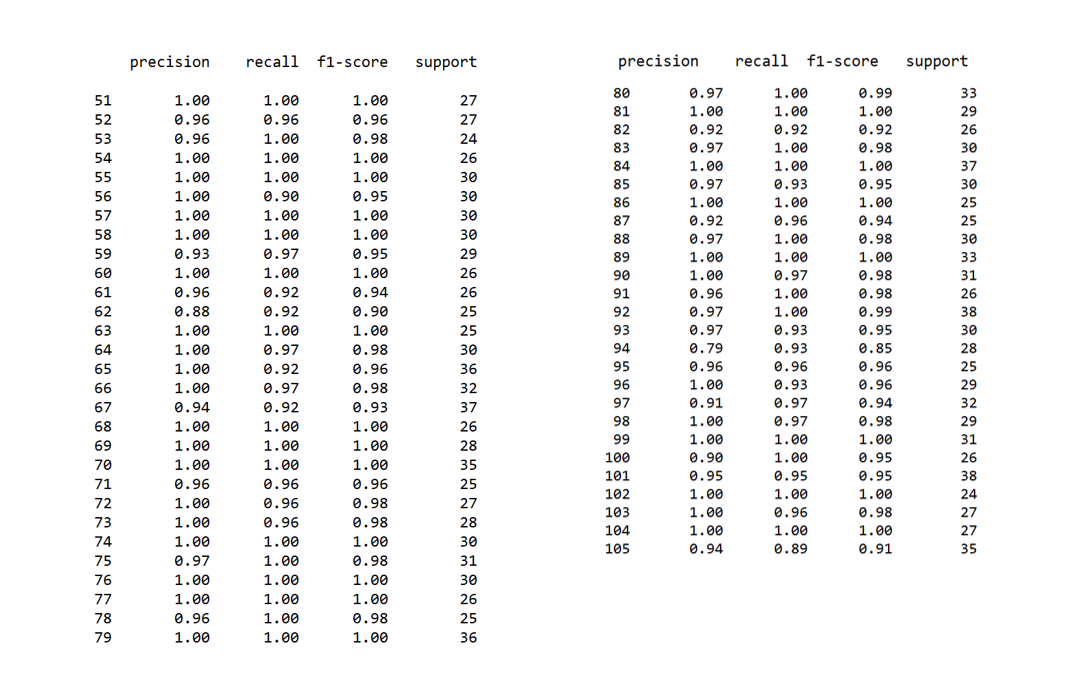
\includegraphics[width=1.1\textwidth]{/clasif2}}
	\caption{Calidad de las clasificaciones obtenidas para cada usuario de la segunda base de datos.}
	\label{clasif2}
\end{table}	

\newpage


\section{Base de datos completa}\label{appe:A3}

% \vfill
% \begin{center}


\begin{table}[h]{
%		\centering
		
		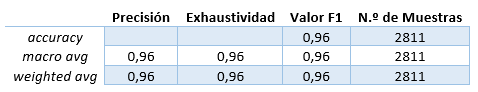
\includegraphics[width=1\textwidth]{/medias}}
	\caption{Calidad de las clasificaciones obtenidas para la base de datos completa.}
	\label{report_}
\end{table}	


%\vfill

\begin{figure}[h]{
		%\centering
		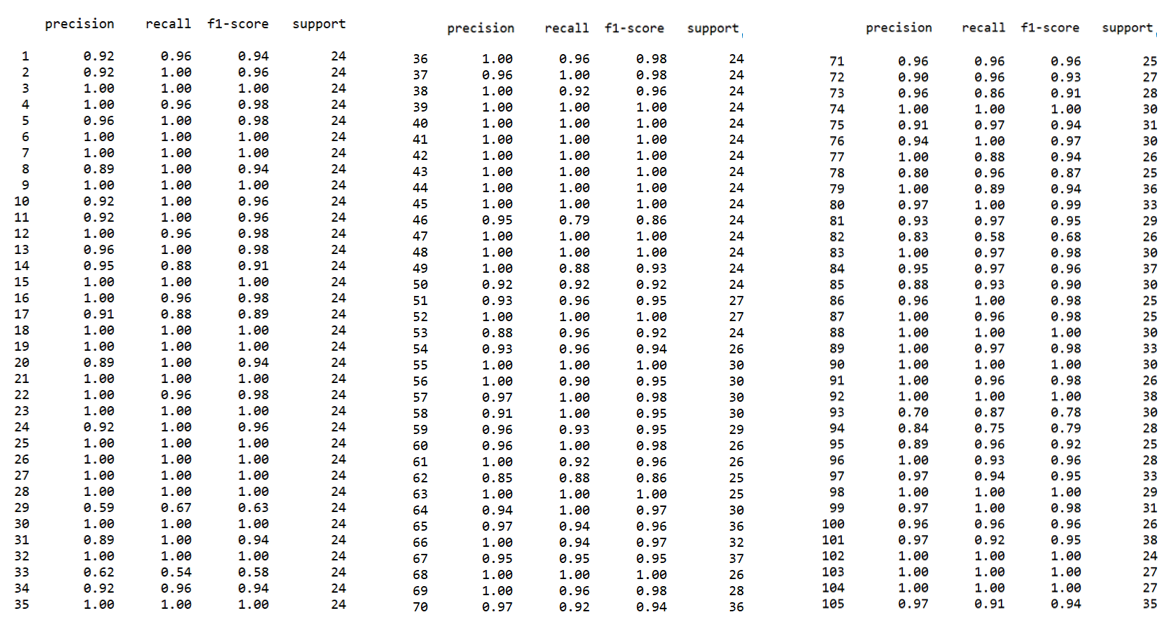
\includegraphics[width=1\textwidth]{/clasif_}}
	\caption{Calidad de las clasificaciones obtenidas para cada usuario de la base de datos completa.}
	\label{clasif_todo}
\end{figure}

%\end{center}
%\vfill
